
\documentclass{report}

\usepackage{amsmath}
\usepackage{amssymb}
\usepackage{cite}
\usepackage{titlepic}
\usepackage{graphicx}
\usepackage{url}
\usepackage{xfrac}
\usepackage{tabto}
\usepackage{caption}
\usepackage{nameref}

\NumTabs{10}
\graphicspath{{./images/}}
\setlength\parindent{0pt}
\NewDocumentCommand{\chapref}{s m}{Chapter~\ref{#2}\IfBooleanF{#1}{ (\nameref{#2})}}





\begin{document}






\titlepic{
\includegraphics[scale=0.5]{DIT_logocol}}
\title{The Problem with Roast Beef}
\author{Jerry Kiely\\
  \\
  School of Mathematical Sciences\\
  Dublin Institute of Technology\\
  Dublin 8\\
  \\
  \texttt{d16126734@mydit.ie}}
\date{\today}
\maketitle







\tableofcontents







\begin{abstract}
In this paper we will write a mathematical model, based on the heat equation, 
in order to verify some well known facts about roasting a piece of meat. We 
will derive an analytical solution, compute values from the analytic solution, 
compare these with values from a numerical solution, and discuss conclusions.
\end{abstract}




















\chapter{Introduction}

In this paper we will construct a mathematical model for roasting a piece of meat, 
assumed to be spherical, based on the heat equation:\bigskip

\[ \frac{\partial T}{\partial t} = \alpha \frac{\partial^2 T}{\partial x^2} \]\medskip

in order to verify a number of facts, such as:\bigskip

\begin{itemize}

\item The roasting time $T$ is proportional to $W^{\frac{3}{2}}$, where $W$ is 
      the weight of the meat
\item After the meat has been removed from the oven, the center temperature 
      continues to rise around $5 - 10\,^{\circ}\mathrm{C}$

\end{itemize}\medskip


We will make a number of assumptions in order to simplify our model:\bigskip

\begin{itemize}

\item The meat is initially at room temperature - this forms the initial condition 
      of the solution

\item The roast is spherical - in truth the roast is not spherical, but by making 
      that assumption we can simplify the problem, and by assuming spherical 
      symmetry we can simplify it even further

\item The meat is homogenous - i.e. it has uniform (constant) density and heat 
      parameters which are not functions of the radius or time

\item There are no changes in the structure of the meat during cooking - so this is 
      not a function of the radius or time either 

\item The temperature in the room and the oven are uniform - there are no variations 
      in temperature at different points at the surface of the meat

\end{itemize}




















\chapter{Mathematical Model}




\section{The Equation}

Recall the heat equation:\bigskip

\[ \frac{\partial T}{\partial t} = \alpha \frac{\partial^2 T}{\partial x^2}, \qquad 0 \leq x \leq L, \qquad t \geq 0 \]\medskip

where $T(x, t)$ is the temperature at the point $x$ and the time $t$, and where $\alpha$ is the 
\emph{heat diffusivity} given by:\bigskip

\[ \alpha = \frac{k}{\rho . c} \]\medskip

where $k$ is the \emph{thermal conductivity}, $\rho$ is the \emph{density}, and $c$ is the 
\emph{specific heat capacity}. As we assume the meat is spherical, we transform the heat equation into spherical 
coordinates (see figure \ref{fig:sc}), and the heat equation becomes:\bigskip

\begin{figure}
\centering
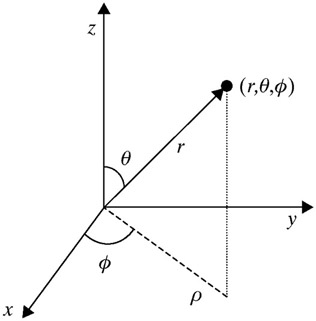
\includegraphics[scale = 0.25]{spherical-coordinates}
\caption{Spherical Coordinates}
\label{fig:sc}
\end{figure}

\[ 
\frac{\partial T}{\partial t} = \alpha 
\Bigg[ 
\frac{1}{r^2} \frac{\partial}{\partial r} \left( r^2 \frac{\partial T}{\partial r} \right)
 + \frac{1}{r^2 sin \theta} \frac{\partial}{\partial \theta} \left( sin \theta \frac{\partial T}{\partial \theta} \right)
 + \frac{1}{r^2 sin^2 \theta} \frac{\partial}{\partial \phi} \left( \frac{\partial T}{\partial \phi} \right)
\Bigg]
\]\medskip

By assuming spherical symmetry, that the temperature only depends on the distance from the centre, i.e. the 
temperature does not depend on $\theta$ or $\phi$, the equation simplifies even further:\bigskip

\[ 
\frac{\partial T}{\partial t} = \alpha \frac{1}{r^2} \frac{\partial}{\partial r} \left( r^2 \frac{\partial T}{\partial r} \right), \qquad 0 \leq r \leq R, \qquad  t \geq 0 
\]\medskip

where $R$ is the radius of the meat.




\section{The Boundary Conditions}

In order to solve our problem we introduce the following boundary conditions:


\subsection{Newton cooling boundary condition at the surface}

Newton's Law of Cooling states that \emph{the rate of change of the temperature of an object is proportional 
to the difference between its own temperature and the temperature of the surrounding medium} ~\cite{wiki:nlc}. 
In equation form, for  $r = R$:\bigskip

\[ -k \frac{\partial T}{\partial r}(R, t) = h (T(R, t) - T_S) \]\medskip

where $k$ is the \emph{thermal conductivity} mentioned earlier, $h$ is the \emph{heat transfer 
coefficient}, and $T_S$ is the temperature of the surrounding medium (the oven or the room). 
So we have:\bigskip

\[ -k \frac{\partial T}{\partial r}(R, t) \]\medskip

is the rate at which the temperature changes on the surface and:\bigskip

\[ h (T(R, t) - T_S) \]\medskip

is the difference between the surface temperature and the temperature of the surrounding medium.



\subsection{Zero-flux boundary condition at the centre}

At $r = 0$ there is no heat transfer in the negative direction. In other words, the temperature has a 
minimum at the centre of the meat, i.e. the first derivative of the temperature with respect to $r$ is 
zero:\bigskip

\[ \frac{\partial T}{\partial r}(0, t) = 0 \]




\section{The Initial Condition}

The initial condition is that the temperature of the roast is room temperature ($T_0$):\bigskip

\[ T(r, 0) = T_0 \]




\section{Scaling}

We will now scale, or non-dimensionalise, the above equations in order to allow us to concentrate on the 
relationship between the important parameters, and also to simplify the analysis of our model. The way we 
do this is to divide each physical parameter by some typical values. For example, in the case of $r$ we 
divide it by the radius $R$ of the meat:\bigskip

\[
\overline{r} = \frac{r}{R}, \qquad 0 \leq \overline{r} \leq 1
\]\medskip

and in the case of $T$ we divide it by $1^{\circ}\mathrm{C}$:\bigskip

\[
\overline{T} = \frac{T}{T^*}, \qquad T^* = 1^{\circ}\mathrm{C}
\]\medskip

and in the case of $t$ we divide it by a value $t^*$, the value of whhich will be decided later:\bigskip

\[
\overline{t} = \frac{t}{t^*} 
\]\medskip

We now transform the PDE, BCs, and IC based on these new variables:



\subsection{Scaling the PDE}

With respect to the LHS we get:\bigskip

\begin{eqnarray*} 
\frac{\partial T}{\partial t} 
& = & \frac{\partial (\overline{T} T^*)}{\partial (\overline{t} t^*)} \\
& = & \frac{T^*}{t^*} \frac{\partial \overline{T}}{\partial \overline{t}}
\end{eqnarray*}\medskip

and with respect to the RHS we get:\bigskip

\begin{eqnarray*} 
\alpha \frac{1}{r^2} \frac{\partial}{\partial r} \left( r^2 \frac{\partial T}{\partial r} \right) 
& = & \alpha \frac{1}{\overline{r}^2 R^2} \frac{\partial}{\partial (\overline{r} R)} \left( \overline{r}^2 R^2 \frac{\partial (\overline{T} T^*)}{\partial (\overline{r} R)} \right) \\
& = & \frac{\alpha T^*}{R^2} \frac{1}{\overline{r}^2} \frac{\partial}{\partial \overline{r}} \left( \overline{r}^2 \frac{\partial \overline{T}}{\partial \overline{r}} \right)
\end{eqnarray*}\medskip

so our equation becomes:\bigskip

\begin{eqnarray*} 
\frac{T^*}{t^*} \frac{\partial \overline{T}}{\partial \overline{t}} 
& = & \frac{\alpha T^*}{R^2} \frac{1}{\overline{r}^2} \frac{\partial}{\partial \overline{r}} \left( \overline{r}^2 \frac{\partial \overline{T}}{\partial \overline{r}} \right) \\
\frac{\partial \overline{T}}{\partial \overline{t}} 
& = & \frac{\alpha t^*}{R^2} \frac{1}{\overline{r}^2} \frac{\partial}{\partial \overline{r}} \left( \overline{r}^2 \frac{\partial \overline{T}}{\partial \overline{r}} \right) \\
& = & A \frac{1}{\overline{r}^2} \frac{\partial}{\partial \overline{r}} \left( \overline{r}^2 \frac{\partial \overline{T}}{\partial \overline{r}} \right)
\end{eqnarray*}\medskip

where $A$ has the value:\bigskip

\[
A = \frac{\alpha t^*}{R^2}
\]\medskip

We can now decide on a value for $t^*$ by setting $A$ equal to $1$:\bigskip

\begin{eqnarray*} 
\frac{\alpha t^*}{R^2} & = & 1 \\
 \therefore \qquad t^* & = & \frac{R^2}{\alpha}
\end{eqnarray*}\medskip

which simplifies our equation considerably. To recover physical time we will need to multiply 
$t$ by $t^*$



\subsection{Scaling the BCs}

With respect to the Newton cooling boundary condition we get:\bigskip

\begin{eqnarray*} 
                                        -k \frac{\partial T}{\partial r} & = & h (T(R, t) - T_S) \\
        -k \frac{\partial (\overline{T} T^*)}{\partial (\overline{r} R)} & = & h (T^* \overline{T}(1, \overline{t}) - T_S) \\
   \frac{- k T^*}{R} \frac{\partial \overline{T}}{\partial \overline{r}} & = & h (T^* \overline{T}(1, \overline{t}) - T_S) \\
                     \frac{\partial \overline{T}}{\partial \overline{r}} & = & \frac{- h R}{k} (\overline{T}(1, \overline{t}) - \frac{T_S}{T^*}) \\
                     \frac{\partial \overline{T}}{\partial \overline{r}} & = & -Bi (\overline{T}(1, \overline{t}) - \overline{T_S})
\end{eqnarray*}\medskip

where $Bi$ is the Biot number, a parameter used frequently in heat transfer problems. It gives a 
measure of the ratio of heat conductivity / transfer - both at the surface and inside the body of 
the object being modelled.\bigskip

\[
Bi = \frac{h R}{k} 
\]\medskip

If $Bi$ is very small, this implies that $k$ (the thermal conductivity) is very large, and / or $h$ 
(the heat transfer coefficient) is very small, which would mean the meat would heat very fast, and the 
temperature would be uniform throughout.\bigskip

With respect to the Zero-flux boundary condition we get:\bigskip

\begin{eqnarray*}  
                                    \frac{\partial T}{\partial r}(0, t) & = & 0 \\
    \frac{\partial (\overline{T} T^*)}{\partial (\overline{r} R)}(0, t) & = & 0 \\
\frac{T^*}{R} \frac{\partial \overline{T}}{\partial \overline{r}}(0, t) & = & 0 \\
   \therefore \frac{\partial \overline{T}}{\partial \overline{r}}(0, t) & = & 0 
\end{eqnarray*} 


\subsection{Scaling the IC}

With respect to the initial condition we get:\bigskip

\begin{eqnarray*} 
\overline{T}(r, 0) & = & \frac{T_0}{T^*} \\\\
                   & = & \overline{T_0}
\end{eqnarray*}\medskip

We may now drop the bars from subsequent calculations, with the understanding that all variables are now 
dimensionless



\section{Transforming the equation}

We now make the transformation $u(r, t) = T(r, t) - T_S$. For our PDE we get the following for the LHS:\bigskip

\begin{eqnarray*} 
              \frac{\partial T}{\partial t} & = & \frac{\partial (u + T_S)}{\partial t} \\
                                            & = & \frac{\partial (u)}{\partial t} + \frac{\partial (T_S)}{\partial t} \\
                                            & = & \frac{\partial u}{\partial t} 
\end{eqnarray*}\medskip

and the following for the RHS:\bigskip

\begin{eqnarray*} 
A \frac{1}{r^2} \frac{\partial}{\partial r} \left( r^2 \frac{\partial T}{\partial r} \right) 
& = & A \frac{1}{r^2} \frac{\partial}{\partial r} \left( r^2 \frac{\partial (u + T_S)}{\partial r} \right) \\
& = & A \frac{1}{r^2} \frac{\partial}{\partial r} \left( r^2 \frac{\partial u}{\partial r} \right) \\
& = & A \Bigg[  \frac{\partial^2 u}{\partial r^2} + \frac{2}{r} \frac{\partial u}{\partial r} \Bigg] 
\end{eqnarray*}\medskip

combining both we get:\bigskip

\begin{eqnarray*} 
\frac{\partial u}{\partial t} & = & A \Bigg[  \frac{\partial^2 u}{\partial r^2} + \frac{2}{r} \frac{\partial u}{\partial r} \Bigg] 
\end{eqnarray*}\medskip

for the BCs and IC we get the following:\bigskip

\begin{eqnarray*} 
\frac{\partial u}{\partial r}(1, t) & = & -Bi \cdot u(1, t) \\
\frac{\partial u}{\partial r}(0, t) & = & 0 \\\\
                            u(r, 0) & = & T_0 - T_S
\end{eqnarray*}\medskip


\section{Summary}

Our model can now be written as follows:\bigskip

\begin{eqnarray*} 
      \frac{\partial u}{\partial t} & = & A \Bigg[  \frac{\partial^2 u}{\partial r^2} + \frac{2}{r} \frac{\partial u}{\partial r} \Bigg], \qquad 0 \leq r \leq 1, \qquad t \geq 0 \\
\frac{\partial u}{\partial r}(1, t) & = & -Bi \cdot u(1, t) \\
\frac{\partial u}{\partial r}(0, t) & = & 0 \\\\
                            u(r, 0) & = & T_0 - T_S
\end{eqnarray*}\medskip

where our variables are:\bigskip

\begin{itemize}

\item $R$       \tab the radius of the spherical piece of meat

\item $r$       \tab the scaled (dimensionless) distance from the centre of the meat

\item $t$       \tab the scaled (dimensionless) time

\item $T(r, t)$ \tab the scaled (dimensionless) temperature

\item $u(r, t)$ \tab $u(r, t) = T(r, t) - T_S$

\end{itemize}\medskip

and our parameters are:\bigskip

\begin{itemize}

\item $T_0$    \tab the initial temperature

\item $T_S$    \tab the temperature of the surrounding medium 

\item $Bi$     \tab the ratio of heat transfer properties 

\item $\alpha$ \tab the heat diffusivity of the meat

\item $k$      \tab the thermal conductivity of the meat

\item $\rho$   \tab the density of the meat

\item $c$      \tab the specific heat capacity of the meat

\item $h$      \tab the heat transfer coefficient

\item $m$      \tab the weight of the meat

\end{itemize}\medskip

Equipped with all of the above we can now proceed with solving our problem.




















\chapter{Analytical Solution}



\section{The solution}

We are now in a position to solve this system. Let $u(r, t) = X(r)T(t)$. Substituting this into our system, 
it becomes:\bigskip

\begin{eqnarray*} 
X(r)T^{\prime}(t) & = & X^{\prime\prime}(r)T(t) + \frac{2}{r}X^{\prime}(r)T(t) \\
\frac{T^{\prime}(t)}{T(t)} & = & \frac{X^{\prime\prime}(r)}{X(r)} + \frac{2}{r}\frac{X^{\prime}(r)}{X(r)}
\end{eqnarray*}\medskip

As the LHS and RHS are functions of $t$ and $r$ respectively, both the LHS and the RHS are set equal 
to a seperation constant $-\lambda$:\bigskip

\begin{eqnarray*} 
\frac{T^{\prime}(t)}{T(t)} & = & -\lambda \\
\frac{X^{\prime\prime}(r)}{X(r)} + \frac{2}{r}\frac{X^{\prime}(r)}{X(r)} & = & -\lambda
\end{eqnarray*}\medskip

With respect to $T$ we have:\bigskip

\begin{eqnarray*} 
T^{\prime}(t) & = & -\lambda \cdot T(t) \\
         T(t) & = & e^{-\lambda t}
\end{eqnarray*}\medskip

With respect to $X$ we have:\bigskip

\begin{eqnarray*} 
               X^{\prime\prime}(r) + \frac{2}{r}X^{\prime}(r) & = & -\lambda X(r) \\
X^{\prime\prime}(r) + \frac{2}{r}X^{\prime}(r) + \lambda X(r) & = & 0 
\end{eqnarray*}\medskip

This contains a non-constant coefficient. So our system has become:\bigskip

\begin{eqnarray*} 
X^{\prime\prime}(r) + \frac{2}{r}X^{\prime}(r) + \lambda X(r) & = & 0, \qquad 0 \leq r \leq 1 \\
                                                X^{\prime}(1) & = & Bi \cdot X(1) \\
                                                X^{\prime}(0) & = & 0 
\end{eqnarray*}\medskip

If we make a change of variables:

\begin{eqnarray*} 
               Y(r) & = & rX(r) \\
      Y^{\prime}(r) & = & X(r) + rX^{\prime}(r) \\
Y^{\prime\prime}(r) & = & 2X^{\prime}(r) + rX^{\prime\prime}(r) 
\end{eqnarray*}\medskip

This gives us the following:\bigskip

\begin{eqnarray*} 
X^{\prime\prime}(r) + \frac{2}{r}X^{\prime}(r) + \lambda X(r) & = & 0 \\
        rX^{\prime\prime}(r) + 2X^{\prime}(r) + \lambda rX(r) & = & 0 \\
                           Y^{\prime\prime}(r) + \lambda Y(r) & = & 0 
\end{eqnarray*}\medskip

For our boundary conditions, from the above, for $r = 1$ we have:\bigskip

\begin{eqnarray*} 
                           Y(1) & = & X(1) \\
                  Y^{\prime}(1) & = & X(1) + X^{\prime}(1) \\
       \therefore X^{\prime}(1) & = & Y^{\prime}(1) - Y(1) \\\\
\therefore Y^{\prime}(1) - Y(1) & = & -Bi \cdot Y(1) \\
                  Y^{\prime}(1) & = & Y(1) - Bi \cdot Y(1) \\
                  Y^{\prime}(1) & = & (1 - Bi)Y(1)
\end{eqnarray*}\medskip

and for $r = 0$ we have:\bigskip

\begin{eqnarray*} 
Y^{\prime}(0) & = & X(0) + 0 \cdot X^{\prime}(0) \\
              & = & X(0) 
\end{eqnarray*}\medskip

but $X(0)$ is unknown so instead we use:\bigskip

\begin{eqnarray*} 
Y(0) & = & 0 \cdot X(0) \\ 
     & = & 0 
\end{eqnarray*}\medskip

So our system becomes:\bigskip

\begin{eqnarray*} 
Y^{\prime\prime}(r) + \lambda Y(r) & = & 0, \qquad 0 \leq r \leq 1 \\
                     Y^{\prime}(1) & = & (1 - Bi)Y(1) \\
                              Y(0) & = & 0 
\end{eqnarray*}\medskip

which is a Sturm-Liouville problem. Solving the auxilary quadratic equation:\bigskip

\begin{eqnarray*} 
m^2 + \lambda & = & 0 \\
          m^2 & = & -\lambda \\
            m & = & \pm \sqrt{-\lambda} 
\end{eqnarray*}\medskip

if $\lambda < 0$:\bigskip

\[
Y(r) = A e^{m_1r} + B e^{m_2r}
\]\medskip

which never works in this context. If $\lambda > 0$:\bigskip

\begin{eqnarray*} 
   m & = & \pm i \sqrt{\lambda} \\
Y(r) & = & A \sin(\sqrt{\lambda_1}r) + B \cos(\sqrt{\lambda_2}r)
\end{eqnarray*}\medskip

setting $r = 0$ we get:\bigskip

\begin{eqnarray*} 
           Y(0) & = & A \sin(0) + B \cos(0) \\
                & = & B \\
                & = & 0 \\
   \therefore B & = & 0 \\
\therefore Y(r) & = & A \sin(\sqrt{\lambda}r) \\
  Y^{\prime}(r) & = & A \sqrt{\lambda} \cos(\sqrt{\lambda}r) 
\end{eqnarray*}\medskip

and setting $r = 1$ we get:\bigskip

\begin{eqnarray*} 
                                           Y(1) & = & A \sin(\sqrt{\lambda}) \\
                                  Y^{\prime}(1) & = & A \sqrt{\lambda} \cos(\sqrt{\lambda}) \\
                                   (1 - Bi)Y(1) & = & (1 - Bi) A \sin(\sqrt{\lambda}) \\
          A \sqrt{\lambda} \cos(\sqrt{\lambda}) & = & (1 - Bi) A \sin(\sqrt{\lambda}) \\\\
    \frac{\sqrt{\lambda}}{\tan(\sqrt{\lambda})} & = & 1 - Bi \\
1 - \frac{\sqrt{\lambda}}{\tan(\sqrt{\lambda})} & = & Bi 
\end{eqnarray*}\medskip

the solutions of which are the eigenvalues of the problem. Proceeding with the 
solution, we recover $X(r)$:\bigskip

\begin{eqnarray*} 
X(r) & = & \frac{Y(r)}{r} \\
     & = & \frac{A \sin(\sqrt{\lambda}r)}{r} 
\end{eqnarray*}\medskip

We are now in a position to write $u(r, t)$ as an infinite sum of eigenfunction products:\bigskip

\begin{eqnarray*} 
u(r, t) & = & \sum_{n = 1}^{\infty} X_n(r)T_n(t) \\
        & = & \sum_{n = 1}^{\infty} c_n  e^{-\lambda_n t} \frac{A \sin(\sqrt{\lambda_n}r)}{r} \\
        & = & \sum_{n = 1}^{\infty} c_n  e^{-\lambda_n t} \frac{\sin(\sqrt{\lambda_n}r)}{r}
\end{eqnarray*}\medskip

Here we have absorbed $A$ into the Fourier coefficients of the infinite sum. Now recovering 
$T(r, t)$:\bigskip

\begin{eqnarray*} 
T(r, t) & = & T_S + u(r, t) \\
        & = & T_S + \sum_{n = 1}^{\infty} c_n  e^{-\lambda_n t} \frac{\sin(\sqrt{\lambda_n}r)}{r} 
\end{eqnarray*}\medskip

at $t = 0$:\bigskip

\begin{eqnarray*} 
                                                               T(r, 0) & = & T_S + \sum_{n = 1}^{\infty} c_n \frac{\sin(\sqrt{\lambda_n}r)}{r} \\
                                                                       & = & T_0 \\
\therefore \sum_{n = 1}^{\infty} c_n \frac{\sin(\sqrt{\lambda_n}r)}{r} & = & T_0 - T_S
\end{eqnarray*}\medskip

In order to find the Fourier coefficients we make use of the orthogonality of the eigenfunctions:\bigskip

\begin{eqnarray*} 
\sum_{n = 1}^{\infty} c_n \sin(\sqrt{\lambda_n}r) \sin(\sqrt{\lambda_m}r) 
  & = & (T_0 - T_S) \sin(\sqrt{\lambda_m}r) r \\
\int_0^1 \sum_{n = 1}^{\infty} c_n \sin(\sqrt{\lambda_n}r) \sin(\sqrt{\lambda_m}r) dr 
  & = & (T_0 - T_S) \int_0^1 \sin(\sqrt{\lambda_m}r) r dr \\
\int_0^1 c_m \sin^2(\sqrt{\lambda_m}r) dr 
  & = & (T_0 - T_S) \int_0^1 \sin(\sqrt{\lambda_m}r) r dr \\
c_m \left( \frac{2\sqrt{\lambda_m} + \sin(2\sqrt{\lambda_m})} {4\sqrt{\lambda_m}} \right) 
  & = & (T_0 - T_S) \left( \frac{\sin(\sqrt{\lambda_m}) - \sqrt{\lambda_m}\cos(\sqrt{\lambda_m})} {\lambda_m} \right) \\
c_m 
  & = & (T_0 - T_S) \frac{1}{\sqrt{\lambda_m}} \left( \frac{4 (\sin(\sqrt{\lambda_m}) - \sqrt{\lambda_m}\cos(\sqrt{\lambda_m}))} {2\sqrt{\lambda_m} + \sin(2\sqrt{\lambda_m})} \right)
\end{eqnarray*}\medskip

Putting this into our equation, we get:\bigskip

\begin{eqnarray*} 
T(r, t) & = & T_S + (T_0 - T_S) \sum_{m = 1}^{\infty} C_m  e^{-\lambda_m t} \frac{\sin(\sqrt{\lambda_m}r)}{\sqrt{\lambda_m}r}
\end{eqnarray*}\medskip

where:\bigskip

\[ 
C_m = \frac{4 (\sin(\sqrt{\lambda_m}) - \sqrt{\lambda_m}\cos(\sqrt{\lambda_m}))} {2\sqrt{\lambda_m} + \sin(2\sqrt{\lambda_m})}
\]\medskip

Note that the above equation for $T(r, t)$ is not valid for $r = 0$, but because we know that:\bigskip

\[
\lim_{x \to 0} \frac{\sin(x)}{x} = 1
\]\medskip

we can rewrite it for the centre as:\bigskip

\[
T_{centre}(t) = \lim_{r \to 0} T(r, t) = T_S +(T_0 - T_S) \sum_{m = 1}^{\infty} C_m  e^{-\lambda_m t} 
\]


\section{The values}

We are now in a position to approximate values for the cooking problem by taking partial sums of the infinite series 
solution. First lets define some values to use:\bigskip

\begin{itemize}

\item $T_0$    \tab $20^{\circ}\mathrm{C}$

\item $T_S$    \tab $180^{\circ}\mathrm{C}$ 

\item $k$      \tab $0.42$ W/mK

\item $\rho$   \tab $1000$ kg/$m^3$

\item $c$      \tab $2921$ J/mK

\item $h$      \tab $50$ W/$m^2$K

\item $m$      \tab $1.5$ kg

\end{itemize}\medskip

We earlier showed that:\bigskip

\begin{eqnarray*} 
1 - \frac{\sqrt{\lambda}}{\tan(\sqrt{\lambda})} & = & Bi 
\end{eqnarray*}\medskip

the solutions of which are the eigenvalues of the problem. By rearranging the above, we can use Maple to find 
eigenvalues as the intersections of the LHS and the RHS of the below equation  (see figure \ref{fig:ev} for a 
visualisation):\bigskip 

\begin{figure}[b]
\centering
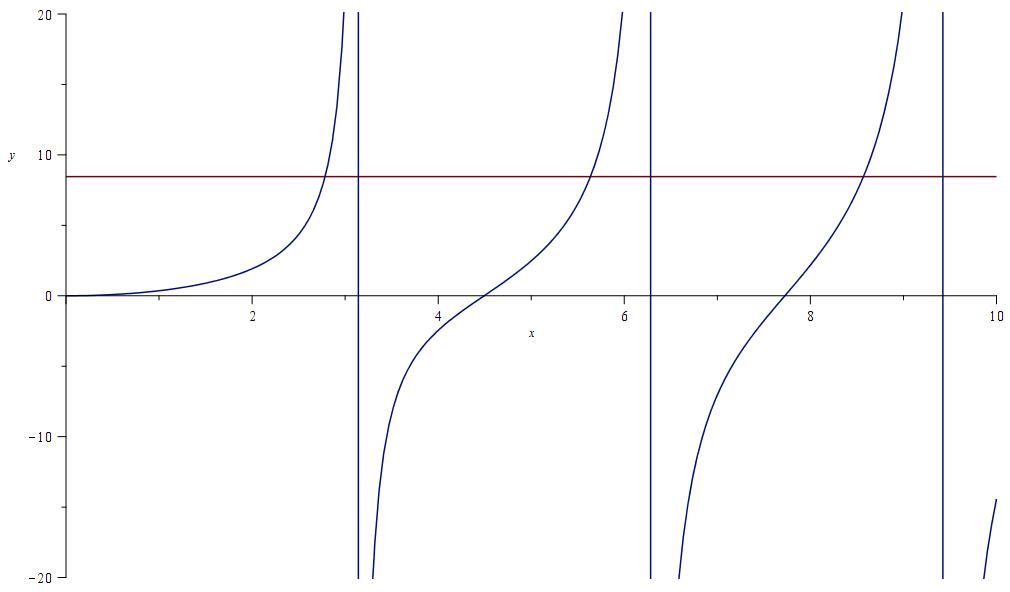
\includegraphics[scale = 0.15]{eigenvalues}
\caption{Plots of $\tan(\sqrt{\lambda})$ and $\frac{\sqrt{\lambda}}{1 - Bi}$}
\label{fig:ev}
\end{figure}

\begin{eqnarray*} 
\tan(\sqrt{\lambda}) & = & \frac{\sqrt{\lambda}}{1 - Bi} 
\end{eqnarray*}\medskip

\begin{table}[h]
\centering
\begin{tabular}{ r | r | r }
$m$ & $\lambda_m$ & $C_m$ \\
\hline
1 &  2.784 &  1.901 \\
2 &  5.636 & -1.667 \\
3 &  8.569 &  1.407 \\
4 & 11.568 & -1.182 \\
5 & 14.609 &  1.003 \\
\end{tabular}
\caption{Eigenvalues and corresponding coefficients}
\label{tab:ec}
\end{table}

We calculate the first five eigenvalues and corresponding coefficients using maple (see table \ref{tab:ec}). 
From these we calculate the cooking time for a medium-rare roast (when the temperature at the centre reaches 
$60^{\circ}\mathrm{C}$) to be $66$ minutes approximately, and for a well-done roast (when the temperature at 
the centre of the roast reaches $70^{\circ}\mathrm{C}$) to be $73$ minutes approximately.\bigskip 

\begin{figure}[h]
\centering
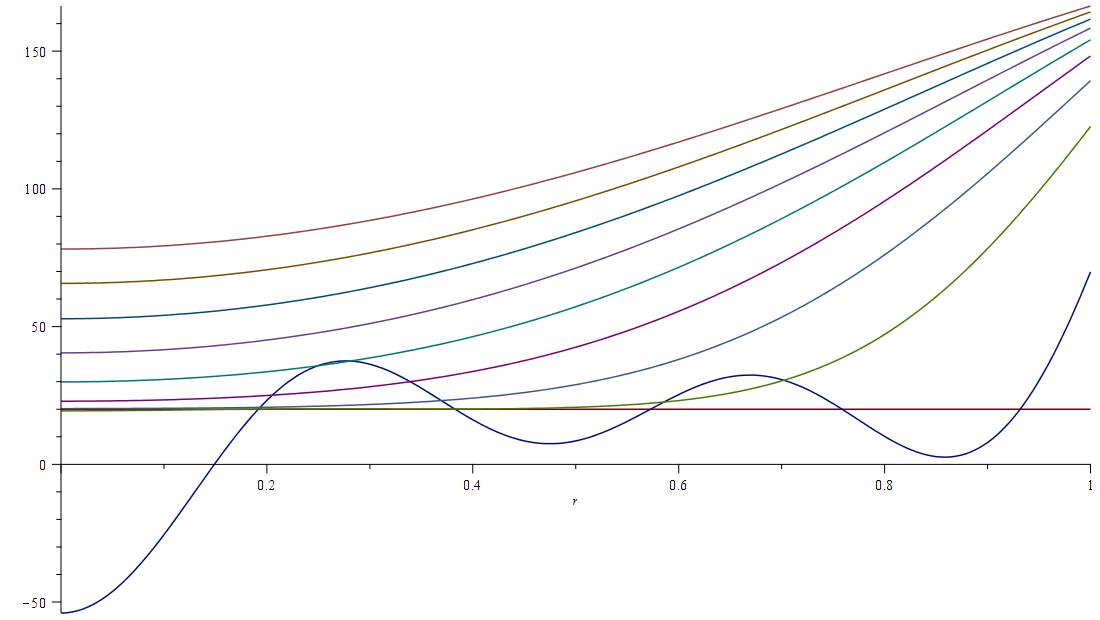
\includegraphics[scale = 0.15]{temperature-distribution-in-radius-analytic}
\caption{The temperature distribution at different times}
\label{fig:td}
\end{figure}

See figure \ref{fig:td} for a plot of temperature distribution for different points over time in the roast. 
The oscilating line is for $t = 0$ and is due to inaccuracy when the infinite sum is approximated by a finite 
number of terms.\bigskip 

\begin{figure}[h]
\centering
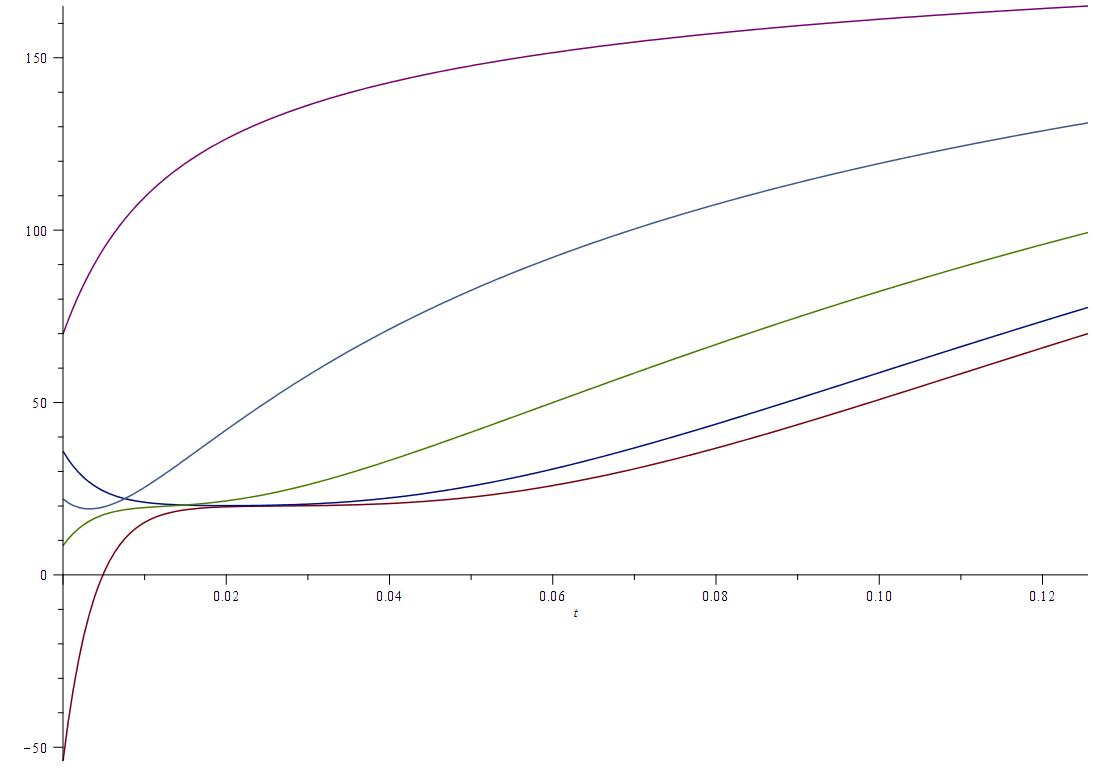
\includegraphics[scale = 0.15]{temperature-evolution-in-time-analytic}
\caption{The temperature at different points in the roast}
\label{fig:te}
\end{figure}

Figure \ref{fig:te} is a plot of the temperature evolution over time at different points in the roast. As can 
be seen, from both plots, the analytic solution doesn't seem to behave well for small $t$, and this is due to 
the fact that we are taking a finite sum of what is an an infinite series. By increasing the number of terms 
in the sum - by calculating more eigenvalues and corresponding coefficients - we can increase the accuracy, 
but $t = 0$ will always be pretty inaccurate and not behave very well.\bigskip 

\begin{figure}[h]
\centering
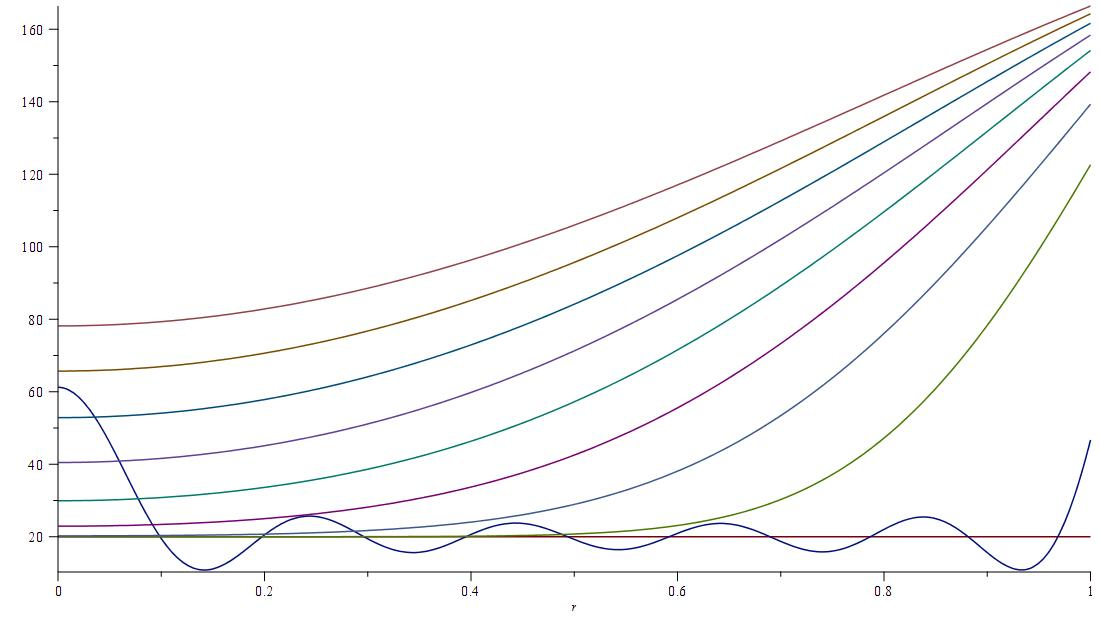
\includegraphics[scale = 0.15]{temperature-distribution-in-radius-double-analytic}
\caption{The temperature distribution at different times - using ten terms}
\label{fig:tdd}
\end{figure}

Indeed, by doubling the number of eigenvalues and coefficients, and by increasing the sum to ten terms, our 
approximation does indeed improve, but the exhibitted oscilatory behaviour around $t = 0$ increases - in fact, 
the number of oscilations doubles (see figure \ref{fig:tdd}).\bigskip

\begin{figure}[h]
\centering
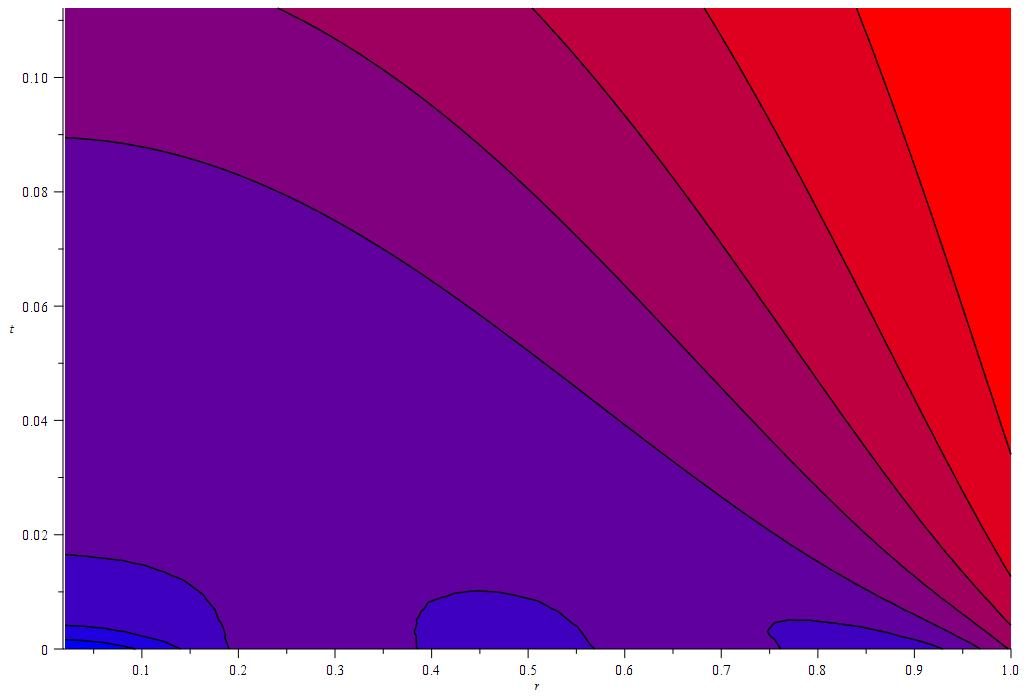
\includegraphics[scale = 0.15]{contour-plot-analytic}
\caption{A contour plot of temperature as a function of position and time}
\label{fig:cp}
\end{figure}

Figure \ref{fig:cp} is a contour plot of the temperature as a function of both radius and time - with the colour 
red representing hot regions and blue representing cold. As can be seen from the contour plot, our solution 
exhibits some strange behaviour - for example, the temperature from the centre to the surface appears to oscilate 
periodically for small $t$. Once again, because we are taking a finite sum as an approximation we are observing 
strange results.\bigskip





















\chapter{Numerical Solution}\label{chap:numerical-solution}

We now look at a numerical solution to the problem. We will use Maple, and specifically \emph{pdsolve}. We give it 
the PDE, the BCs and the IC, and calculate values and plot the results. We will use the same values for the parameters 
we used in the previous section.\bigskip

\begin{figure}[h]
\centering
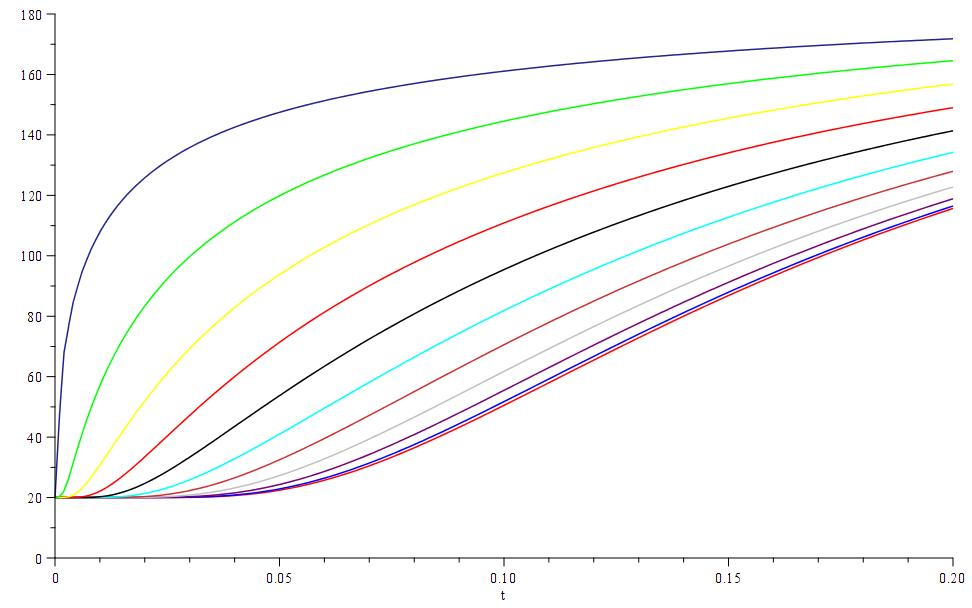
\includegraphics[scale = 0.15]{temperature-evolution-in-time-numeric}
\caption{The temperature at different points in the roast during cooking}
\label{fig:ten}
\end{figure}

To begin with we will look at the temperature evolution at different points in the roast during cooking. In figure 
\ref{fig:ten} we see a plot of the temperature over a two hour period with each curve representing a different point in 
the roast.\bigskip

\begin{figure}[h]
\centering
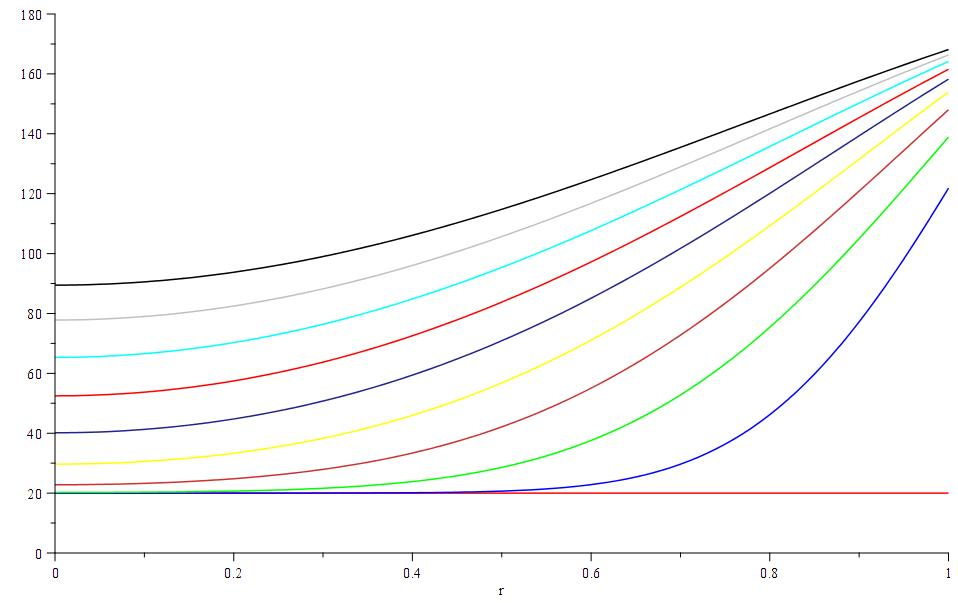
\includegraphics[scale = 0.15]{temperature-distribution-in-radius-numeric}
\caption{The temperature distribution at different times during cooking}
\label{fig:tdn}
\end{figure}

Next we look at the temperature variation across the radius 
of the roast over the cooking period. In figure \ref{fig:tdn} we see a plot of the temperature at different points in the 
radius at different times. We can see the temperature rises sharply as you get closer to the surface.\bigskip

\begin{figure}[h]
\centering
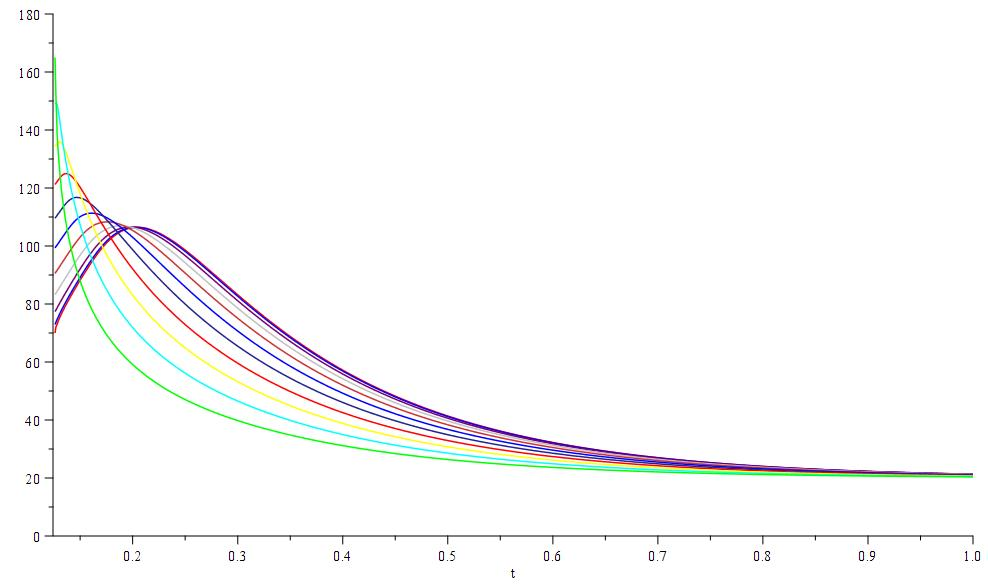
\includegraphics[scale = 0.15]{temperature-distribution-in-radius-cooling-numeric}
\caption{The temperature distribution at different times during cooling}
\label{fig:tdcn}
\end{figure}

Next we look at the temperature variation across the radius of the roast at different times during cooling. In figure 
\ref{fig:tdcn} we see a plot of the temperature at different points in the radius over time. We can see the temperature 
lowers reasonably uniformly, but the temperature at, and towards, the centre continues to rise for a period after the 
roast has been removed from the oven.\bigskip

\begin{figure}[h]
\centering
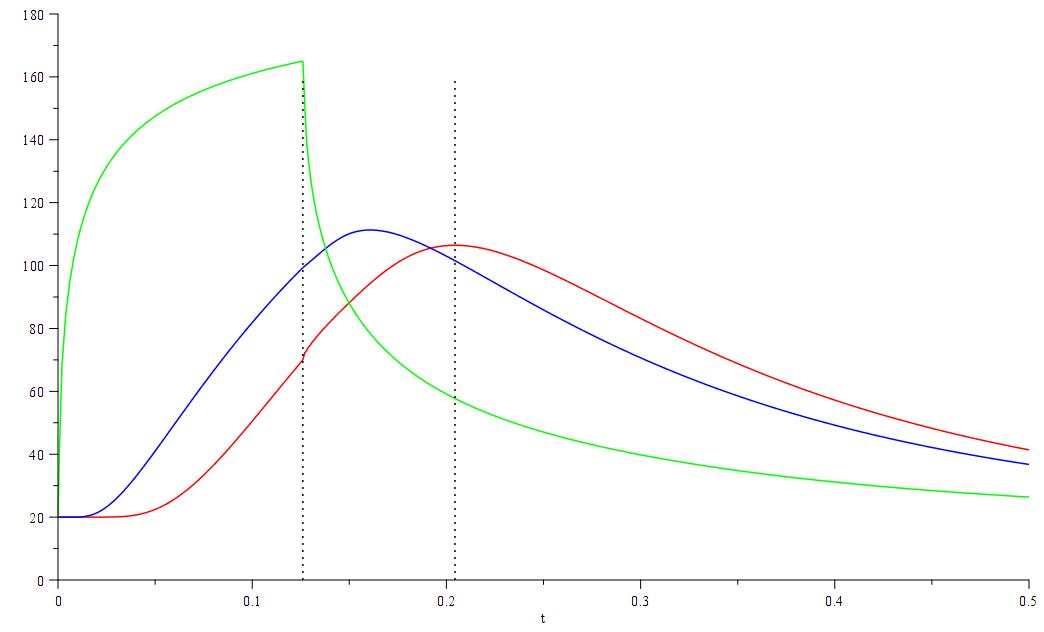
\includegraphics[scale = 0.15]{cooking-and-cooling-numeric}
\caption{Cooking and cooling}
\label{fig:cacn}
\end{figure}

In figure \ref{fig:cacn} we see a plot of the temperature at different points in the radius over time for both cooking 
and cooling. The two vertical lines indicate the point when the centre of the roast (in red) reaches $70^{\circ}\mathrm{C}$ 
and the point when the centre reaches it's maximum.\bigskip

Note the smoothness of these plots around $r = 0$ in comparison with the plots of the analytic solution. We can clearly see 
that, for the cooking phase, the temperature at, and near, the surface rises quickly in comparison with the temperature at, 
and towards, the centre, and the temperature at the centre continues to rise to a maximum after the roast has been taken 
out of the oven.\bigskip























\chapter{Further Work}\label{chap:further-work}

\section{Is cooking time proportional to the weight of the roast?}

\subsection{Analytic solution}

Table \ref{tab:ctvrw} lists the cooking times - the times for the centre to reach $70^{\circ}\mathrm{C}$ - for various 
roast weights using data from the analytic solution:\bigskip

\begin{table}[h]
\centering
\begin{tabular}{ r | r | r | r | r | r }
Weight (kg) & $0.5$ & $1$ & $1.5$ & $2$ & $2.5$ \\
\hline
Cooking time (min) & 37.75 & 57.32 & 73.40 & 87.59 & 100.53 
\end{tabular}
\caption{Roast weight with coresponding cooking time}
\label{tab:ctvrw}
\end{table}

Figure \ref{fig:ctvw} plots the points from the analytic solution with weight raised to the power of $\frac{2}{3}$.\bigskip

\begin{figure}[h]
\centering
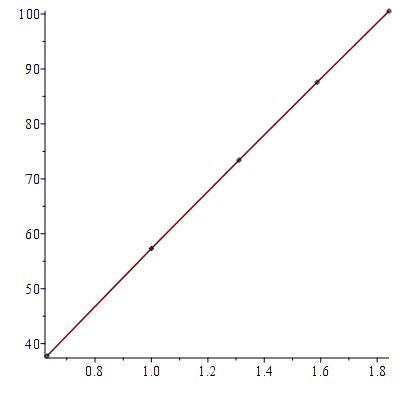
\includegraphics[scale = 0.25]{cooking-time-versus-weight-analytic}
\caption{Cooking time versus weight to the power of $\frac{2}{3}$ (analytic solutuion)}
\label{fig:ctvw}
\end{figure}

\subsection{Numeric solution}

Table \ref{tab:ctvrwn} lists, also for various weights, the cooking times, the time taken for the roast to reach it's 
maximum temperature at the centre after being taken out of the oven, and by how many degrees the temperature of the roast 
rises after ten minutes of cooling using the numeric solution.\bigskip

\begin{table}[h]
\centering
\begin{tabular}{ c | r | r | r }
Weight (kg) & Cooking time & Time to maximum & Temp. rise after $10$ min \\
\hline
$0.5$ & 37.89 & 23.82 & 22.70 \\
\hline
$1$   & 57.54 & 35.78 & 15.68 \\
\hline
$1.5$ & 75.40 & 45.17 & 14.80 \\
\hline
$2$   & 87.94 & 53.94 & 10.89 \\
\hline
$2.5$ & 100.93 & 61.60 & 9.71 
\end{tabular}
\caption{Roast weight with coresponding cooking time}
\label{tab:ctvrwn}
\end{table}

Figure \ref{fig:ctvwn} plots the points from the numeric solution with weight raised to the power of $\frac{2}{3}$.\bigskip

\begin{figure}[h]
\centering
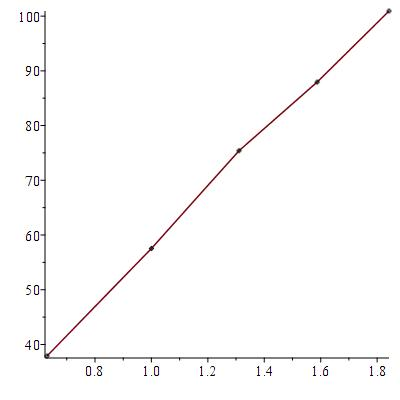
\includegraphics[scale = 0.25]{cooking-time-versus-weight-numeric}
\caption{Cooking time versus weight to the power of $\frac{2}{3}$ (numeric solutuion)}
\label{fig:ctvwn}
\end{figure}

\subsection{Conclusion}

As can be seen from both plots the relationship is clear, but the line going through the points from the numeric solution is 
less straight.



















\chapter{Model Discussion and Conclusions}




\section{Model performance}

Did our model reproduce the predictions detailed in the introduction?\bigskip

\begin{itemize}

\item The roasting time $T$ is proportional to $W^{\frac{3}{2}}$, where $W$ is 
      the weight of the meat
\item After the meat has been removed from the oven, the center temperature 
      continues to rise around $5 - 10\,^{\circ}\mathrm{C}$

\end{itemize}\medskip

For the first of our predictions we confirmed this to be the case in \chapref{chap:further-work}.\bigskip

As for the second of our predictions - does the temperature at the centre continue to rise after the meat has been removed 
from the oven - we have shown this to be the case in \chapref{chap:numerical-solution}. Indeed our numerical solution has 
shown that the predicted temperature rise has been underestimated.\bigskip

So our predictions have been confirmed by both models.




\section{Comparison of solutions}

With respect to our two solutions, we ask two questions:\bigskip 

\begin{itemize}

\item Were our two approaches consistent?

\item Which of the two was more accurate?

\end{itemize}\medskip

By plotting both solutions against each other we can get an insight. For example, figure \ref{fig:c1} plots temperature at 
the centre for both the analytic (red dot) and numeric (blue dashed) solution over time:\bigskip

\begin{figure}[h]
\centering
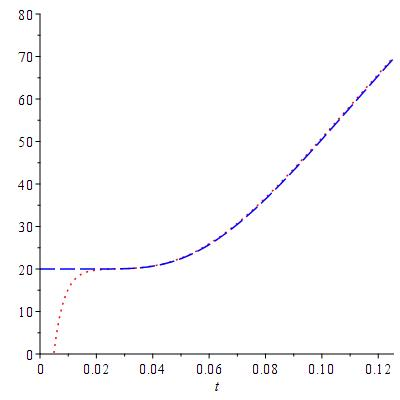
\includegraphics[scale = 0.25]{compare-01}
\caption{Analytic versus Numeric for $r = 0$}
\label{fig:c1}
\end{figure}

Clearly they deviate for $t$ in the neighbourhood of $0$. A similar plot (figure \ref{fig:c2}) for the surface shows more 
consistency:\bigskip

\begin{figure}[h]
\centering
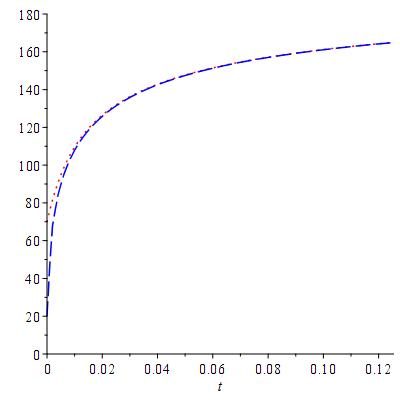
\includegraphics[scale = 0.25]{compare-02}
\caption{Analytic versus Numeric for $r = 1$}
\label{fig:c2}
\end{figure}

The real difference between the solutions can be see if we plot temperature versus radius for $t = 0$ (figure \ref{fig:c3}):\bigskip

\begin{figure}[h]
\centering
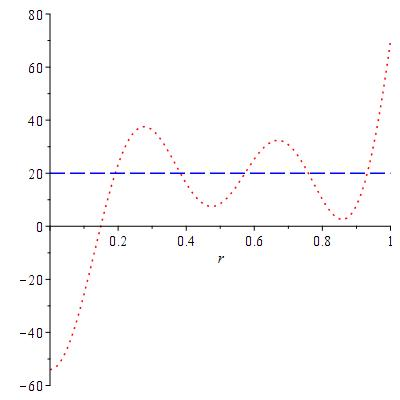
\includegraphics[scale = 0.25]{compare-03}
\caption{Analytic versus Numeric for $t = 0$}
\label{fig:c3}
\end{figure}

But this behaviour improves for $t > 0$, as can be seen if we plot temperature versus radius for 
$t = \frac{t_{cook}}{2}$ (figure \ref{fig:c4}):\bigskip

\begin{figure}[h]
\centering
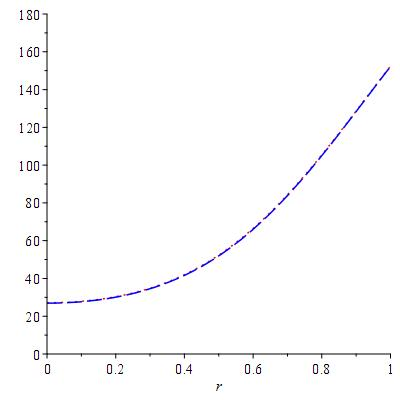
\includegraphics[scale = 0.25]{compare-04}
\caption{Analytic versus Numeric for $t = \frac{t_{cook}}{2}$}
\label{fig:c4}
\end{figure}

So certainly, with the exception of in or around the neighbourhood of $t = 0$, the solutions are very consistent. And 
any issues the analytic solution had around $t = 0$ were resolved by the numeric solution.




\section{Model assumptions}

In truth, many of our assumptions were oversimplifications:\bigskip

\begin{itemize}

\item The roast is spherical - the roast is always pretty irregularly shaped, and it may in fact 
      be more accurate to treat the roast as a cylinder

\item The meat is homogenous - in fact, the meat does not have uniform (constant) density and heat 
      parameters - which would be functions of time and radius

\item There are no changes in the structure of the meat during cooking - this is certainly not the 
      case, and these changes would also be a function of time and radius

\item The temperature in the room and the oven are uniform - this may not be the case in an oven 
      that is not fan assisted

\end{itemize}

All of the parameters used in the model would change over time, and we choose to make these assumptions in order to make 
our model simpler, but further research should make these parameters functions of $t$ and $r$\bigskip



\section{Conclusion}


Qualitatively speaking, the model performs very well. It seems to accurately predict what we expected. And quantitatively 
speaking, the values seem to be consistent - for example, the cooking time for a roast would agree with experience.\bigskip

All in all, for what is a reasonably simple model with some reasonably naive assumptions, the model has performed surprisingly 
well. 












\bibliographystyle{plain}
\bibliography{bibtex/Newtons_Law_Of_Cooling,bibtex/Industrial_Mathematics,bibtex/Applied_Partial_Differential_Equations}{}


\end{document}
